\documentclass[a4paper,12pt]{article}

\usepackage[utf8]{inputenc}
\usepackage{graphicx}
\usepackage{xcolor}
\usepackage{float}

%\usepackage{tgheros}
%\usepackage[defaultmono]{droidmono}

\usepackage{amsmath,amssymb,amsthm,textcomp}
\newcommand{\argmin}{\operatornamewithlimits{argmin}}
\newcommand{\NiceHat}[1]{\expandafter\hat#1} 
\usepackage{enumerate}
\usepackage{enumitem}
\usepackage{multicol}
\usepackage{tikz}
\usetikzlibrary{arrows,calc}
\tikzset{
 >=stealth',
 help lines/.style={dashed, thick},
 axis/.style={<->},
 important line/.style={thick},
 connection/.style={thick, dotted},
}

\usepackage{CJKutf8}

\usepackage{geometry}
\geometry{total={210mm,297mm},
left=25mm,right=25mm,%
bindingoffset=0mm, top=20mm,bottom=20mm}


\linespread{1.3}

\newcommand{\linia}{\rule{\linewidth}{0.5pt}}

% custom theorems if needed
% my own titles
\makeatletter
\renewcommand{\maketitle} {
\begin{center}
\vspace{2ex}
{\LARGE \textsc{\@title}}
\vspace{1ex}
\\
\linia\\
\@author \hfill \@date
\vspace{4ex}
\end{center}
}
\makeatother
%%%

% custom footers and headers
\usepackage{fancyhdr}
\pagestyle{fancy}
\lhead{}
\chead{}
\rhead{}
\lfoot{Inverse Problem Final Report}
\cfoot{Page \thepage}
\rfoot{15M54097}
\renewcommand{\headrulewidth}{0pt}
\renewcommand{\footrulewidth}{0pt}
%


% code listing settings
\usepackage{listings}
\lstset{
    language=Matlab,
    basicstyle=\ttfamily\small,
    aboveskip={1.0\baselineskip},
    belowskip={1.0\baselineskip},
    columns=fixed,
    extendedchars=true,
    breaklines=true,
    tabsize=4,
    prebreak=\raisebox{0ex}[0ex][0ex]{\ensuremath{\hookleftarrow}},
    frame=lines,
    showtabs=false,
    showspaces=false,
    showstringspaces=false,
    keywordstyle=\color[rgb]{0.627,0.126,0.941},
    commentstyle=\color[rgb]{0.133,0.545,0.133},
    stringstyle=\color[rgb]{01,0,0},
    numbers=left,
    numberstyle=\small,
    stepnumber=1,
    numbersep=10pt,
    captionpos=t,
    escapeinside={\%*}{*)}
}


%\renewcommand*\thelstnumber{\arabic{lstnumber}:}

%\DeclareCaptionFormat{mylst}{\hrule#1#2#3}
%\captionsetup[lstlisting]{format=mylst, labelfont=bf, singlelinecheck=off, labelsep=space}

\begin{document}

\title{Advanced Course of Inverse Problem}

\author{NGUYEN T. Hoang - SID: 15M54097}

\date{Fall 2015, W832 Fri. Period 1-2 \\ \hfill Due date: 2016/01/20}

\maketitle
\vspace{-4.5em}
\hspace{5.3em} (\begin{CJK}{UTF8}{min}ホアン\end{CJK})
\vspace{4em}
\section*{Problem}
\begin{itemize}
	\item Given a image of a barcode:
	\begin{figure}[h]
		\centering
		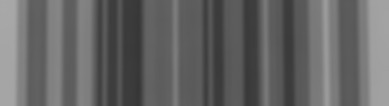
\includegraphics[width=0.5\textwidth]{barcode_b.jpg}
		\caption{A blurred image of a barcode. File name: \texttt{barcode\_b.pgm}}
		\label{fig:blurbar}
	\end{figure}
    \item A matlab program \texttt{decom.m} is available to visualize the intensity distribution of the image.
	\item Explain the observation system $y=Ax$ for this problem.
	\item Build the system matrix A.
	\item Reconstruct with LSM.
	\item Reconstruct with Tikhonov Regulation method.
	\item Reconstruct with TSVD.
	\item Find the best regularization parameter with L-Curve method. 
\end{itemize}
\vspace{4em}
\pagebreak
\section*{Q1: Explain the system and build system matrix}
\setcounter{section}{1}

\textit{Explain the observation system $y = Ax$ and build the system matrix A.} 

\vspace{1.5em}
\noindent
\textbf{Answer:} 
\noindent
The problem in this assignment is to recover barcode data from a given blurred barcode image. Barcode reader can be a phone camera or a specialized device with photosensor and laser light. In this probelm, we only care about data on a perpendicular line with the barcode. Furthermore, the observation ($g(s)$ and true value ($f(t)$) depends only on the displacement $s-t$. Therefore, this problem is a 1-D deconvolution problem:
$$ Ax = b $$
where $A$ is a system matrix describing the convolution, $x$ is a 1-D vector storing the \emph{true} value of the barcode, and b is a 1-D vector storing sensor/camera observation. \\ 

The system formula can be re-written as follow: 
$$ \sum_{j=1}^{n-1} h_{i-j}x_j = b_i $$
where $h_{i-j}$ is a function describing relationship with $x_j$ and $b_i$. Our model for the blur is the Gaussian kernel:
$$ h_{i-j} = \frac{1}{n} \mbox{ exp}\left(-\frac{(i-j)^2}{\sigma^2 n^2} \right) $$

Choose $\sigma = 0.01$, we can construct the convolutional system matrix A as follow:

\begin{lstlisting}[caption={MATLAB code for system matrix A. }]
	% Get length of the observation vector from given c in decom.m
	n = length(c);
	sigma = 0.01;
	A = (1/n) .* toeplitz(exp(-((0:n-1)/(sigma*n)).^2));
	% A is a 380x380 parse matrix.
\end{lstlisting}

\begin{figure}[h]
	\centering
	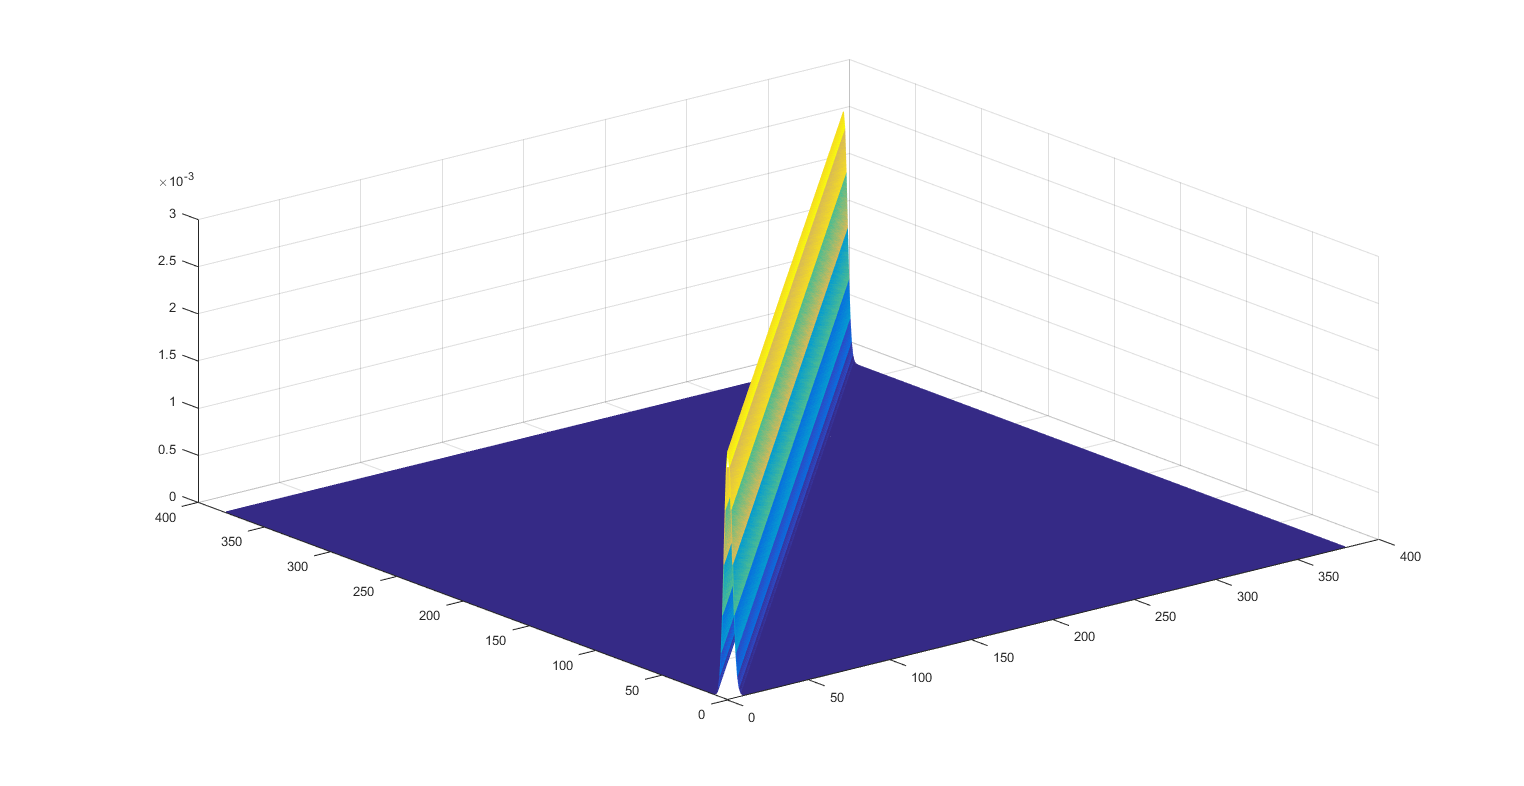
\includegraphics[width=0.8\textwidth]{matA.png}
	\caption{Mesh plot of system matrix A}
	\label{fig:matA}
\end{figure}
 




\section*{Q2: Reconstruct with LSM.}
\setcounter{section}{1}

\textit{Reconstruct the barcode with Least Square Method.} 

\vspace{1.5em}
\noindent
\textbf{Answer:} 
\noindent
The Least Square Solution is given by this following formula:
$$ x_{ls} = (A^TA)^{-1}A^Ty $$
This is the unique $x \in \mathcal{R}^n$ that minimizes $||Ax-y||$.
\\
In MATLAB, we can also compute $x_{ls}$ with the \emph{backslash operator}. However, I will use aforementioned approximation formula.

\begin{lstlisting}[caption={MATLAB code for Least Square Method.}]
	% Approximate Least Square Solution
	x_ls = pinv(A' * A) * (A' * c);
	figure; plot(x_ls); title('LSM Reconstruction');
\end{lstlisting}

\begin{figure}[h]
	\centering
	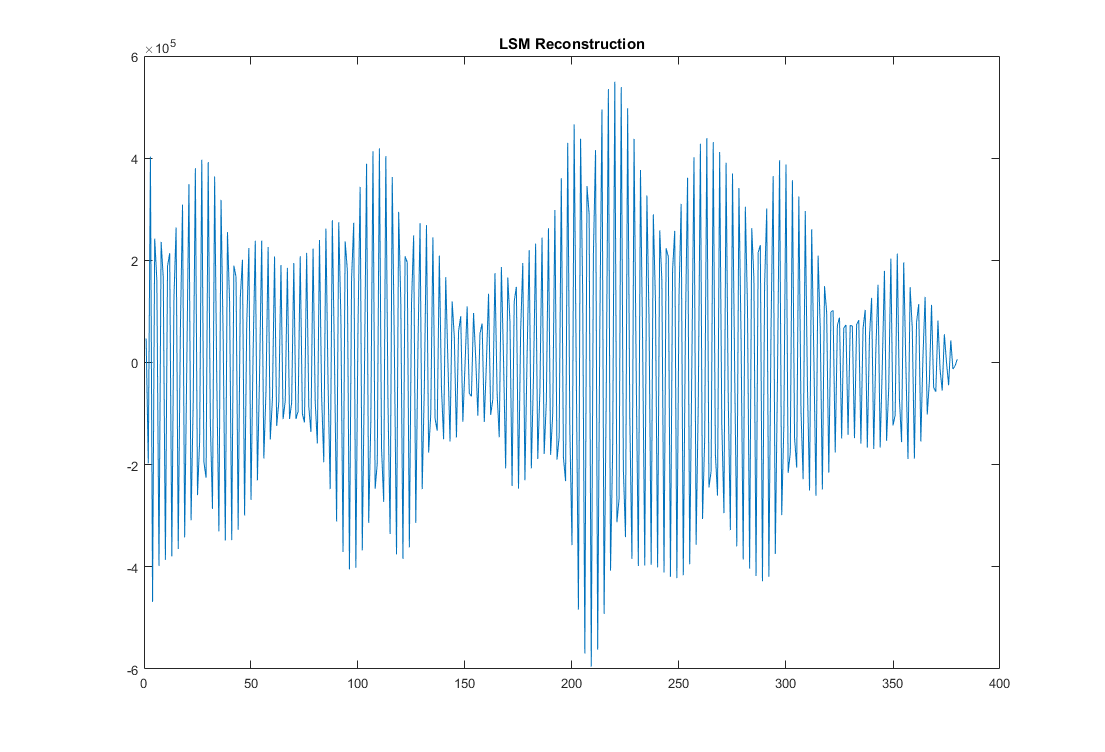
\includegraphics[width=0.8\textwidth]{LSM_graph.png}
	\caption{LSM Reconstruction result.}
	\label{fig:lsm}
\end{figure}







\section*{Q3: Reconstruct with Tikhonov Regulation Method.}
\setcounter{section}{1}

\textit{Reconstruct the barcode with Tikhonov Regulation Method.} 

\vspace{1.5em}
\noindent
\textbf{Answer:} 
\noindent
The Tikhonov Regulation is given by this following formula:
$$ x_{tk} = \argmin_x (||Ax-b||^2_2 + \lambda^2||x||^2_2) $$
or $x_\lambda$, a solution corresponds with a real number $\lambda$, is given by:
$$ x_{\lambda} = (A^TA + \lambda^2I)^{-1}A^Tb $$
where A is the system matrix and b is our observation. In MATLAB, I choose $\lambda = 3.5$, we can compute the value $x_{\lambda}$ as follow:

\begin{lstlisting}[caption={MATLAB code for Tikhonov Regulation with $\lambda = 3.5$.}]
	% Tikhonov Regulation solution 
	lambda = 3.5;
	x_tk = pinv(A' * A + lambda^2 * eye(n)) * (A' * c);
	figure; plot(x_tk); title('Tikhonov Regulation Reconstruction');
\end{lstlisting}

\begin{figure}[H]
	\centering
	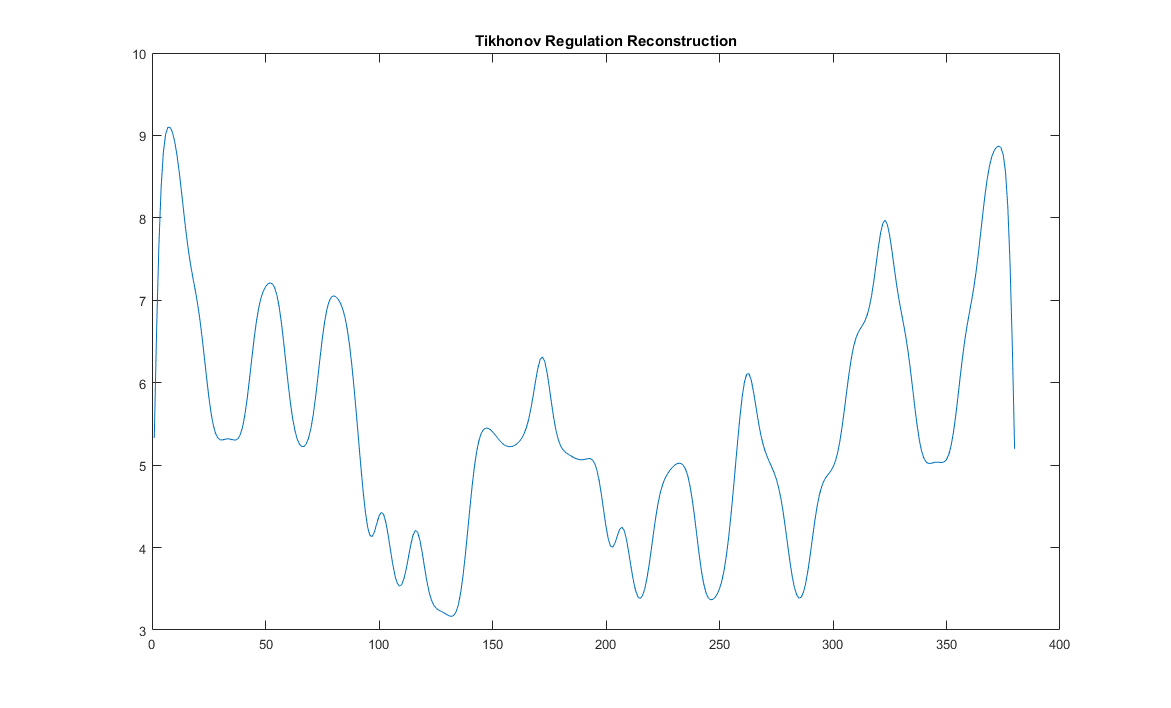
\includegraphics[width=0.8\textwidth]{TK_graph.png}
	\caption{Tikhonov Regulation Reconstruction result.}
	\label{fig:tk}
\end{figure}


\pagebreak
\section*{Q4: Reconstruct with TSVD.}
\setcounter{section}{1}

\textit{Reconstruct the barcode with TSVD.} 

\vspace{1.5em}
\noindent
\textbf{Answer:} 
\noindent
The system matrix can be decomposed using Single Value Decomposition:
$$ A = UDV^T, $$
where:
$$ D = \mbox(diag)(d_1,...,d_n). $$
The $\NiceHat{x^{(k)}}$ estimation with a parameter $k$ is given by:
$$  \NiceHat{x^{(k)}} = \Sigma_{j=1}^{k} \frac{1}{d_j} (u^T_j b)v_j  $$
where $d_j$ is elements of the diagnal, $u_j$ is row j of matrix $U$, $v_j$ is row j of matrix V, and b is our observation. In MATLAB, I choose $k = 40$, we can estimate the solution as follow:

\vspace{2em}
\begin{lstlisting}[caption={MATLAB code for TSVD with $k = 40$.}]
	% TSVD  
	[U,D,V] = svd(A);
	d = diag(D);
	r = find(d > eps, 1, 'last');
	x_tsvd = zeros(n,r);
	normX = zeros(r,1);
	disp = zeros(r,1);
	for k = 1:r
		x_tsvd(:,k) = V(:,1:k)*diag(1./d(1:k))*U(:,1:k)'*c;
		normX(k) = norm(x_tsvd(:,k));
		disp(k) = norm(c-A*x_tsvd(:,k));
	end
	figure; plot(x_tsvd(:,40)); title('TSVD Reconstruction, k = 40');
\end{lstlisting}
\vspace{2em}

The TSVD by far is the best construction that I have obtained. By choosing $k=40$, the result shows intensity for each bar clearly. In my observation, we can use this result and the JAN-8 barcode standard to derive the item this barcode refers to.

\begin{figure}[H]
	\centering
	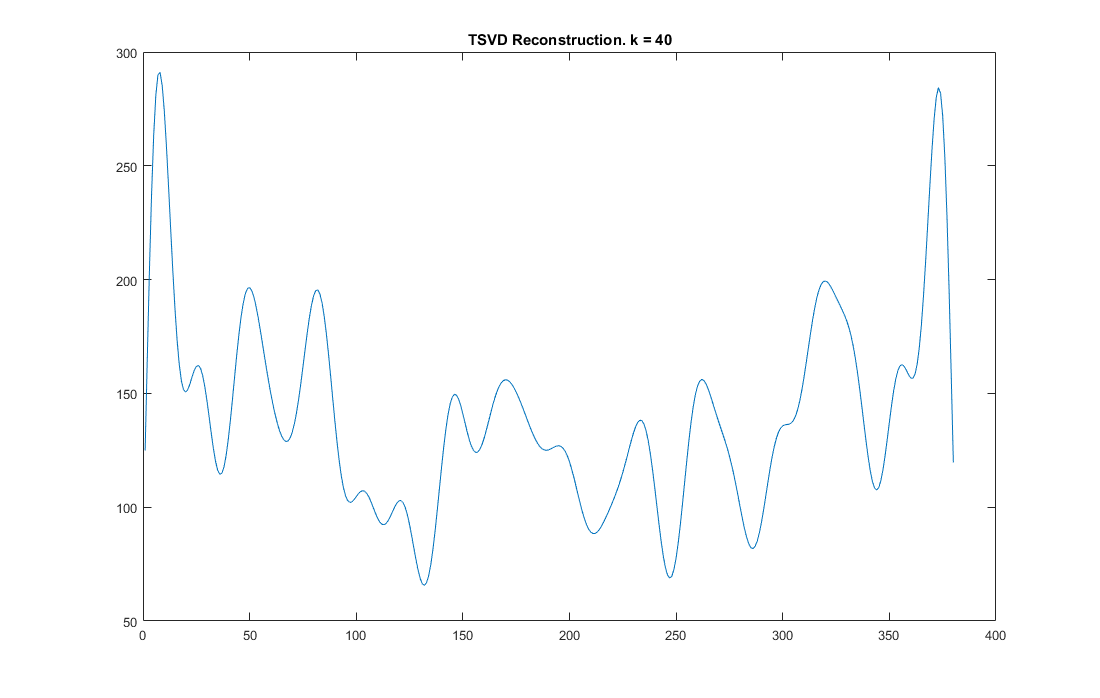
\includegraphics[width=0.8\textwidth]{TSVD_graph.png}
	\caption{TSVD Reconstruction result.}
	\label{fig:tsvd}
\end{figure}

\vspace{-2em}
\section*{Q5: Best regularization parameter with L-Curve.}
\setcounter{section}{1}

\textit{Find the best regularization parameter of TR and TSVD with L-Curve.} 

\vspace{1em}
\noindent
\textbf{Answer:} $\lambda = 0.6$ and $k = 178$.
\vspace{-1em}
\noindent

\begin{lstlisting}[caption={MATLAB code for ploting Tikhonov Regularization L-Curve.}]
	% L-Curve Tikhonov
	x_tk_l = zeros(n,100);
	x_tk_norm = zeros(100,1);
	x_tk_disp = zeros(100,1);
	it = 1;
	for i = 0.1:0.1:10
	    x_tk_l(:,it) = pinv(A' * A + i^2 * eye(n))*A'*c;
	    x_tk_norm(it) = norm(x_tk_l(:,it));
	    x_tk_disp(it) = norm(c-A*x_tk_l(:,it));
	    it = it + 1;
	end
	figure;
	loglog(x_tk_norm,x_tk_disp,'c.','MarkerSize', 20,'MarkerEdgeColor',[0 .5 .5]);
	hold on
	loglog(x_tk_norm,x_tk_disp,'k-','LineWidth', 2)
	hold off
	text(1650.463759, 865.547447,'  \lambda = 0.6');
	title('L-Curve Tikhonov Regulation');
\end{lstlisting}

\begin{figure}[H]
	\centering
	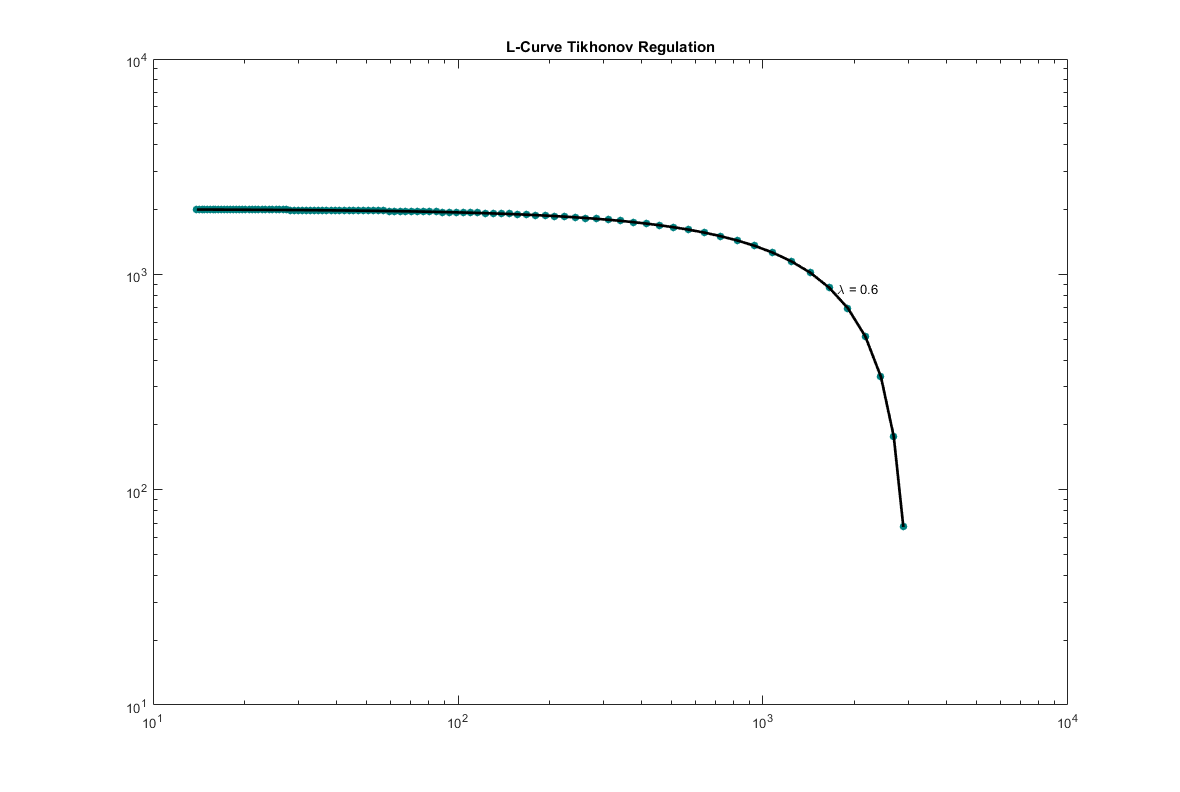
\includegraphics[width=0.8\textwidth]{lcurve_tk.png}
	\caption{L-Curve result Tikhonov Regulation.}
	\label{fig:ltk}
\end{figure}

\vspace{-2em}

\begin{lstlisting}[caption={MATLAB code for ploting Tikhonov Regularization L-Curve.}]
	figure;
	loglog(normX,discr,'c.','MarkerSize', 10,'MarkerEdgeColor',[.5 0 0]);
	hold on
	loglog(normX,discr,'k-','LineWidth', 2)
	hold off
	text(11503.53877, 4.551855,'     k = 178');
	title('L-Curve TSVDS Regulation');
\end{lstlisting}

\begin{figure}[H]
	\centering
	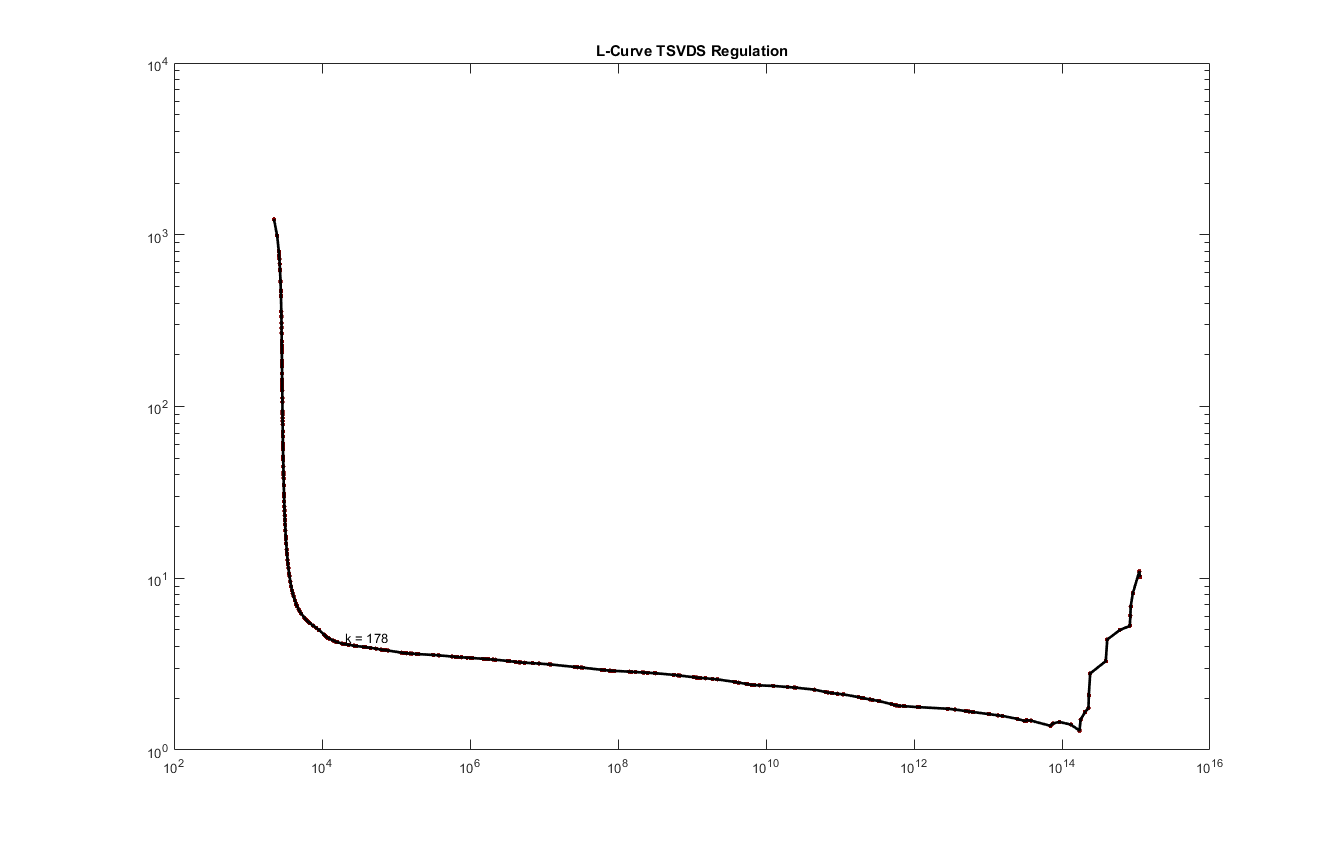
\includegraphics[width=0.74\textwidth]{lcurve_tsvd.png}
	\caption{L-Curve result TSVD.}
	\label{fig:ltsvd}
\end{figure}

\end{document}
